\subsection{Mollweide Projektion}
\label{sec:Mollweiden}
Bei der Mollweiden Projektion wird die Erde als Oval dargestellt. Die Mollweiden Projektion ist flächentreu.
Der Äquator und der Nullmeridian werden bei der Mollweiden Projektion maßstabsgetreu wieder gegeben.
Breitenkreise werden bei der Mollweiden Projektion als Geraden dargestellt. Die Längenkreise sind als Ellipsen dargestellt.\\

\begin{figure}[hbtp]
\centering
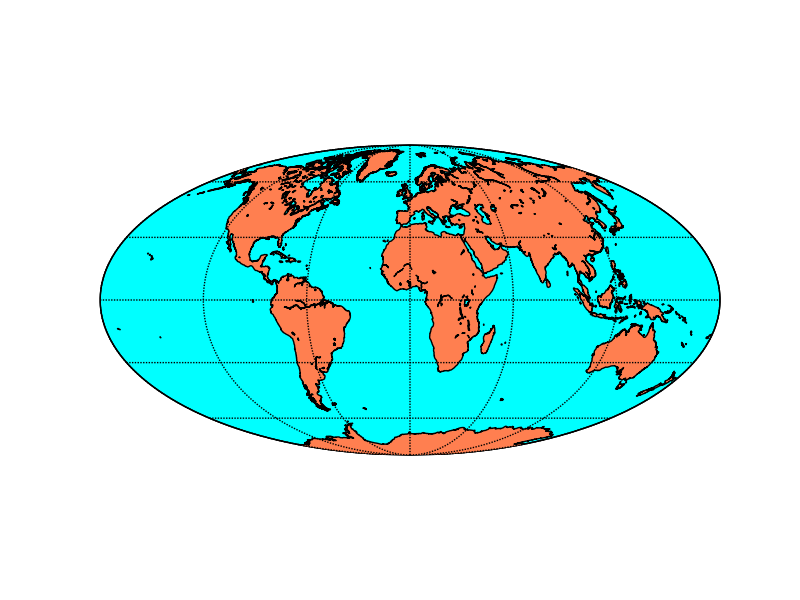
\includegraphics[scale=0.5,origin=c]{/Users/student/seminar/Kartendarstellungen/seminar/moll} \caption{Mollweiden Projektion}
\end{figure}
\newpage 